
%使用XeLaTeX编译
%版权所有,翻版必究
%本文件由程序自动生成,任何修改将被覆盖
%2019 年 01 月 23 日




\FloatBarrier
\section{
初识Qt Quick控件
}\label{s100510}


%begin图片
\begin{figure}[htb] %浮动体 here and top ...
%there must use marginnote ...
\marginnote{\setlength\fboxsep{2pt}\fbox{\footnotesize{\kaishu\figurename\,}\footnotesize{\ref{p000007}}}}\centering %中心对齐
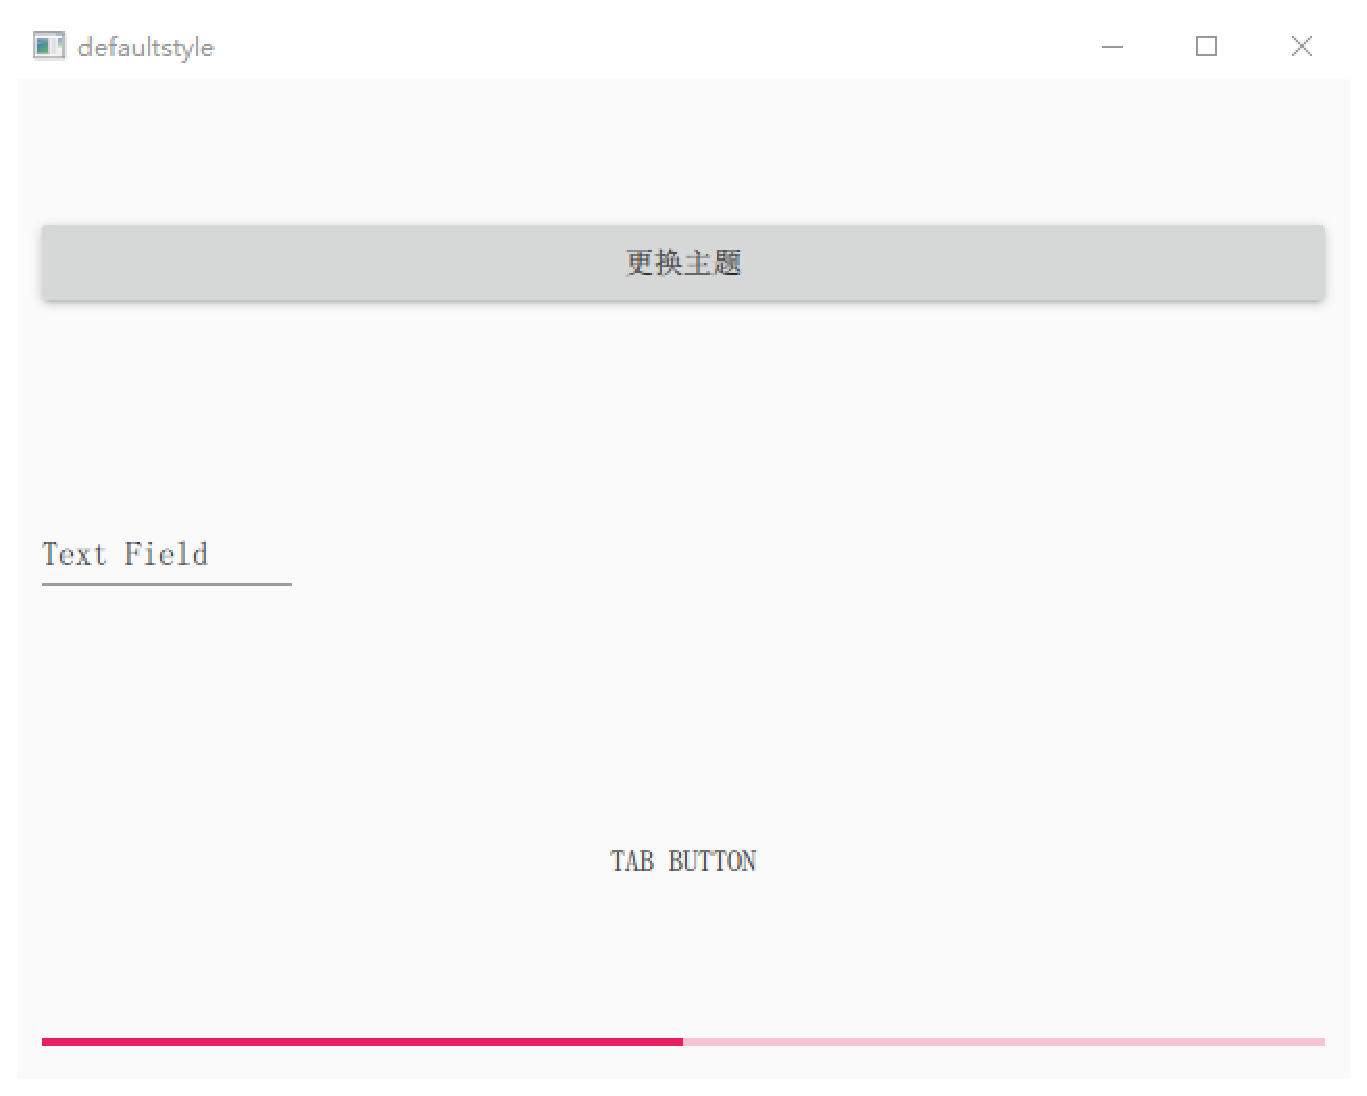
\includegraphics[width=0.95\textwidth]{the_book_image/p000007.eps} %图片路径
\caption{Qt Quick控件及样式!} %标题
\label{p000007} %索引
\end{figure}
%end图片


Qt Quick Controls 2 自Qt 5.7引入。

本书不加特别说明,提到Qt Quick Controls就是指
Qt Quick Controls 2。

Qt Quick Controls 1更多的是沿用传统桌面
的设计风格;而
Qt Quick Controls 2更加现代化并更适用于
移动设备。
并且,Qt Quick Controls 2对于主题和样式
提供了专门的语法支持。

基于这些语法,读者可以轻松的实现样式、内容和结构分离。
即使读者不想在样式上太花费心思,Qt Quick Controls 2也
默认提供了数个艺术级的样式模板。

除了维护老项目,
没有什么理由不采用Qt Quick Controls 2。

本项目的“main.qml”如\filesourcenumbernameone\ \ref{f000035}
所示:

%\begin{spacing}{1.0}
\refstepcounter{filesourcenumber}\label{f000035}    %增加源代码编号
\FloatBarrier                                  %强制完成浮动体布局
\begin{thebookfilesourceone}[escapeinside={(*@}{@*)},
caption=GoodLuck,
title=\filesourcenumbernameone \thefilesourcenumber
]
/*defaultstyle/main.qml*/
import QtQuick 2.9
import QtQuick.Controls 2.3
import QtQuick.Layouts 1.3
import QtQuick.Controls.Material 2.12

Pane {

    id : idRoot
    width: 640;
    height: 480;

    function changeTheme(){
        if(idRoot.Material.theme === Material.Dark ){
            idRoot.Material.theme = Material.Light;
        }else{
            idRoot.Material.theme = Material.Dark;
        }
    }

    ColumnLayout {
        id: idColumn
        anchors.fill: parent

        Button {
            id: idButton
            text: qsTr("更换主题")
            Layout.fillWidth : true
            onClicked: {
                idRoot.changeTheme();
            }
        }

        TextField {
            id: idTextField
            text: qsTr("Text Field")
            Layout.fillWidth : true
        }

        TabButton {
            id: idTabButton
            text: qsTr("Tab Button")
            Layout.fillWidth : true
        }

        ProgressBar {
            id: idProgressBar
            value: 0.5
            Layout.fillWidth : true
        }

    }

}/*~Pane*/(*@\marginpar[\hfill\setlength\fboxsep{2pt}\fbox{\footnotesize{\kaishu\parbox{1em}{\setlength{\baselineskip}{2pt}\filesourcenumbernameone}}\footnotesize{\thefilesourcenumber}}]{\setlength\fboxsep{2pt}\fbox{\footnotesize{\kaishu\parbox{1em}{\setlength{\baselineskip}{2pt}\filesourcenumbernameone}}\footnotesize{\thefilesourcenumber}}}@*)\end{thebookfilesourceone}          %抄录环境
\addtocounter{lstlisting}{-1}   %sub lstlisting counter ...
%\end{spacing}
%main.qml

\begin{itemize}
\item 第21行展示了如何使用Layout;
\item 第28行、第37行、第43行、第49行
展示了使用关联属性\footnote{
Attached Properties。
};
\item 第29\raisebox{0.16ex}{\sourcefonttwo\~{}}31行展示了如何关联一个Qml信号到一个
JavaScript函数;%……
\item 第13\raisebox{0.16ex}{\sourcefonttwo\~{}}19行展示了如何在一个Qml对象里面
使用JavaScript定义
一个槽函数;
\end{itemize}

本案例演示了如何使用Qt Quick Control自带的“Material”样式。

要使用Qt Quick Control自带的样式,需要在QApplication
构造之前调用如\filesourcenumbernameone\ \ref{f000037}
所示的C{\sourcefonttwo{}+}{\sourcefonttwo{}+}代码,以载入配置文件。

%\begin{spacing}{1.0}
\refstepcounter{filesourcenumber}\label{f000037}    %增加源代码编号
\FloatBarrier                                  %强制完成浮动体布局
\begin{thebookfilesourceone}[escapeinside={(*@}{@*)},
caption=GoodLuck,
title=\filesourcenumbernameone \thefilesourcenumber
]
::qputenv("QT_QUICK_CONTROLS_CONF","defaultstyle_qtquickcontrols2.conf");(*@\marginpar[\hfill\setlength\fboxsep{2pt}\fbox{\footnotesize{\kaishu\parbox{1em}{\setlength{\baselineskip}{2pt}\filesourcenumbernameone}}\footnotesize{\thefilesourcenumber}}]{\setlength\fboxsep{2pt}\fbox{\footnotesize{\kaishu\parbox{1em}{\setlength{\baselineskip}{2pt}\filesourcenumbernameone}}\footnotesize{\thefilesourcenumber}}}@*)\end{thebookfilesourceone}          %抄录环境
\addtocounter{lstlisting}{-1}   %sub lstlisting counter ...
%\end{spacing}


配置文件内容如\filesourcenumbernameone\ \ref{f000036}
所示:
%\begin{spacing}{1.0}
\refstepcounter{filesourcenumber}\label{f000036}    %增加源代码编号
\FloatBarrier                                  %强制完成浮动体布局
\begin{thebookfilesourceone}[escapeinside={(*@}{@*)},
caption=GoodLuck,
title=\filesourcenumbernameone \thefilesourcenumber
]
[Controls]
Style=Material
FallbackStyle=Material

[Material]
Theme=Dark(*@\marginpar[\hfill\setlength\fboxsep{2pt}\fbox{\footnotesize{\kaishu\parbox{1em}{\setlength{\baselineskip}{2pt}\filesourcenumbernameone}}\footnotesize{\thefilesourcenumber}}]{\setlength\fboxsep{2pt}\fbox{\footnotesize{\kaishu\parbox{1em}{\setlength{\baselineskip}{2pt}\filesourcenumbernameone}}\footnotesize{\thefilesourcenumber}}}@*)\end{thebookfilesourceone}          %抄录环境
\addtocounter{lstlisting}{-1}   %sub lstlisting counter ...
%\end{spacing}
%defaultstyle_qtquickcontrols2.conf

Qt Quick Control的样式具有继承性。

子控件的样式与父控件一致,
只需要更改父控件的样式,
则子控件的样式跟随父控件变化。












%使用XeLaTeX编译
%版权所有,翻版必究
%本文件由程序自动生成,任何修改将被覆盖
%2019 年 01 月 23 日



